\documentclass[twoside]{article}

\usepackage{epsfig}
\usepackage{amsfonts}
\usepackage{tikz}
\usepackage{amsthm}

\setlength{\oddsidemargin}{0. 25 in}
\setlength{\evensidemargin}{-0. 25 in}
\setlength{\topmargin}{-0. 6 in}
\setlength{\textwidth}{6. 5 in}
\setlength{\textheight}{8. 5 in}
\setlength{\headsep}{0. 75 in}
\setlength{\parindent}{0 in}
\setlength{\parskip}{0. 1 in}

\newcommand{\lecture}[4]{
   \pagestyle{myheadings}
   \thispagestyle{plain}
   \newpage
   \setcounter{page}{1}
   \noindent
   \begin{center}
   \framebox{
      \vbox{\vspace{2mm}
    \hbox to 6. 28in { {\bf STA561:~Probabilistic machine learning \hfill} }
       \vspace{6mm}
       \hbox to 6. 28in { {\Large \hfill #1 (#2)  \hfill} }
       \vspace{6mm}
       \hbox to 6. 28in { {\it Lecturer: #3 \hfill Scribes: #4} }
      \vspace{2mm}}
   }
   \end{center}
   \markboth{#1}{#1}
   \vspace*{4mm}
}

\begin{document}

\lecture{Variational Inference}{11/4/13}{Barbara Engelhardt}{Tracy Schifeling,  Alireza Samany,  and Matt Dickenson}

\section{Introduction}

In this lecture we will  further discuss Variational Inference and then proceed with Loopy Belief Propagation, also known as LBP. In the last lecture we discussed Mean Field Variational Inference and we investigated the matter in the context of univariate Gaussians. In this lecture, we will talk further about Variational Inference in the context of the Ising Model, which is a Markov random field, and then we proceed with Mean Field and Loopy Belief Propagation.  

Let us begin by reviewing Variational Inference.  In Variational Inference, we have our data set as $\mathcal{D}=\{X_1, X_2, \dots, X_n\}$ and we describe both our latent variables, $Z_{1:m}$, and the set of our model parameters, $\theta$, by a single parameter $Z$ such that $Z=\{Z_{1:m}, \theta \}$. 

We are interested at estimating the posterior probability of latent variables given the data, which is $p(Z|X)$. By definition of the conditional distribution, we know that the posterior probability of latent variables given data is equal to the joint distribution of latent variables and data divided by the marginal probability of the data(observed variables). Therefore, we have:

\begin{eqnarray*}
p(Z|X)=\frac{p(Z, X)}{\int_Z{p(Z, X)dZ}}
\end{eqnarray*}

Variational Inference, is another method to compute an approximation to the posterior distribution. In general, computing the posterior distribution for several distributions, such as truncated Gaussians or Gaussians mixture models, can be very hard. This issue obliges us to resort to computing approximations for the posterior distribution. For example, consider the case of Gaussian Mixture Models. Let us assume the standard mixture model where each class specific mean $\mu_k$ is distributed according to $\mu_k \sim \mathcal{N}(0, \tau^2)$, our latent variables $Z_i$ have the distribution $Z_i \sim Mult(\pi)$ for a fixed hyperparameter $\pi$, and the data $X_i$ is distributed as $X_i \sim \mathcal{N}(\mu_k, \Sigma_k)$. So our model will be:

\begin{eqnarray*}
\mu_k &\sim& \mathcal{N}(0, \tau^2)
Z_i &\sim& Mult(\pi)
X_i &\sim& \mathcal{N}(\mu_k, \Sigma_k)
\end{eqnarray*}

which leads to the following expression for the posterior distribution using the chain rule:

\begin{eqnarray*}
p(\mu, Z|X)&=&\frac{\prod_{k=1}^K{p(\mu_k)}x \prod_{i=1}^n{p(Z_i|\pi)x p(Z_i|X_i, \mu_{1:k})}}{\int_{\mu_{1:K}} \Sigma_{Z_{1:n}}\prod_{k=1}^K{p(\mu_k)}x \prod_{i=1}^n{p(Z_i|\pi)x p(Z_i|X_i, \mu_{1:k})}d\mu_{1:K}}
\end{eqnarray*}

The numerator is simple to compute. However, computing the denumerator is exponentially difficult. In addition, the integral in the denumerator is generally not straightforward. These problems serve as our motivation for finding approximate posterior distributions. We will need to tackle the same problem again once we discuss LDA models, which also lead to exponentially hard denumerators. 

Let us return to our previous discussion on the space of possible parametrizations of our original posterior distributions named $\mathcal{M}$. It turns out that if we consider all the values of $Z$ which are consistent with the posterior distribution derived above, we have a theorem that for most models such as Gaussian models and many discrete models, for the given data the $Z$ parameters lie in a convex polytope. 

The immediate advantage of this fact is that we can do optimization over a convex space to find the parameters $Z$. However, the density on the space $M$ might not have a form convenient to optimize as we have previously for the Gaussian Mixture Model. \\

\begin{center}
\begin{picture}(150, 150)(-150, 0)
\put(0, 50){\line(1, 1){50}}
\put(50, 100){\line(1, 0){50}}
\put(100, 100){\line(1, -1){50}}
\put(150, 50){\line(-1, -1){50}}
\put(100, 0){\line(-1, 0){50}}
\put(50, 00){\line(-1, 1){50}}
\put(75, 50){$\mathcal{M}$}
\put(90, 75){. Z}
\makebox(140, -20)[40]{Convex polytope $\mathcal{M}$ conatining the  possible parameter values $Z$}
\end{picture}
\end{center}

Let us review Mean Field in order to fully understand our goal in Variational Inference. Our goal in the Mean Field is to find a fully factorized posterior distribution. We assume an approximation to the posterior in the form of $q(Z)=\prod_{i=1}^m{q(Z_i)}$ and attempt to obtain the following:

\begin{eqnarray*}
\min_{Z}{KL(q(Z)||p(Z|X))} 
\end{eqnarray*}

We should note that each variable is assumed to be independent of the others here. Remember that based on the reverse KL divergence, we need the support of $q(Z)$ to lie entirely in the support of $p(Z|X)$. The marginal independence assumption we imposed here leads us to a parameterization space which is no longer convex as shown in the figure below. However, this new space, called $\mathcal{M}_{MF}$,  turns out to be straightforward to search over when we use  computable expressions for $q(Z_i)$. We should note that it is very possible that the desired $Z^*$ does not lie in $\mathcal{M}_MF$. 

\begin{center}
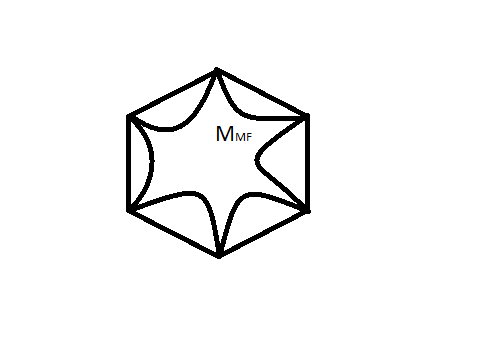
\includegraphics{convexpolytope}
\end{center}

Here we do the optimization above using an unnormalized $p(Z|X)$, but let us look at the optimzation above from an entirely different perspective by using a concept called the Evidence Lower Bound, also known as ELBO. 


\subsection{Evidence Lower Bound}
Let us recall Jensen's Inequality first. According to jensen's Inequality, we know that for a given convex function $f(\cdot)$ we have $E[f(x)] \leq f(E[x])$. This can be derived directly using the definition of expectation and applying the convexity property of $f(\cdot)$. As $\log(x)$ is a convex function, we can apply Jensen's Inequality to it. Let us consider $\log(p(X))$. We have:\\

\begin{eqnarray*}
log(p(X)) &=& \log \int_Z{p(X, Z)}dZ \\
&=& \log \int_Z {p(X, Z)}x \frac{q(Z)}{q(Z)}dZ \\
&=& \log E_q[\frac {p(X, Z)}{q(Z)}] \\
\end{eqnarray*}

Using Jensen's Inequality, we have:

\begin{eqnarray*}
\log(p(X)) &=& \log E_q[\frac {p(X, Z)}{q(Z)}] \ge E_q[\log(\frac {p(X, Z)}{q(Z)})] =E_q[\log(p(X, Z))]-E_q[\log(q(Z))]
\end{eqnarray*}

Let us recall a result we derived in the last lecture:

\begin{eqnarray*}
KL(q|| \~ p)=-E_q[\log(p(Z, X)]+E_q[\log(q(Z)]+\log(p(X)) \Rightarrow KL(q|| \~ p)=-ELBO+\log(p(X))
\end{eqnarray*}

Therefore, ELBO is KL divergence with unnormalized posterior. Since $p(X)$ is independent of $q(Z)$, minimizing the KL divergence is equivalent to minimizing the ELBO. 
Therefore there are two steps to minimize the KL divergence:

\begin{enumerate}
\item Choosing a proposition, $q$,  such that the expectations are computable.
\item Maximize $q(Z)$ with respect to the ELBO in order to obtain the tightest possible approximation to $p(X, Z)$
\end{enumerate}


\section{Ising Model}

% previous section should end with a discussion of ELBO
Before proceeding with variational inference,  it is helpful to review the Ising model.  The main idea behind the Ising model is a lattice of unobserved variables ($x_1, . . . x_n$),  each with its own (noisy) observation ($y_1,  . . . ,  y_n)$).  

For example,  suppose our goal is to reconstruct a denoised image given noisy observations of the pixels.  We can think of the lattice as  the pixels in a black and white image ($x_i \in \{-1,  1\}$),  with a noisy grayscale observation of the pixels ($y_i \in R)$.  More generally,  we wish to draw inferences about the unobserved lattice $X$ from the observed values $Y$.  Figure \ref{ising} illustrates an Ising model for $n=9$,  with the latent nodes colored white and the observed nodes shaded grey.  

\begin{figure}[h!]
\begin{center}
\begin{tikzpicture}
\scriptsize
\foreach \i in {1, . . . , 9}
{
        \pgfmathtruncatemacro{\y}{(\i - 1) / 3};
        \pgfmathtruncatemacro{x}{\i - 3 * \y};
        \pgfmathtruncatemacro{\label}{x + 3 * (2 - \y)};
        \pgfmathtruncatemacro{\labely}{(x + 3 * (2 - \y))*10};
        \node[circle, draw=black, fill=white, minimum size=20]
        (\label) at (1. 5*x, 1. 5*\y) {$x_\label$};
        \node[circle, draw=black, fill=white!80!black, minimum size=20]
        (\labely) at (1. 5*x-0. 8, 1. 5*\y-0. 8) {$y_\label$};
}
% Lattice of X's
\draw (1) -- (2);
\draw (1) -- (4);
\draw (2) -- (3);
\draw (2) -- (5);
\draw (3) -- (6);
\draw (4) -- (5);
\draw (4) -- (7);
\draw (5) -- (6);
\draw (5) -- (8);
\draw (6) -- (9);
\draw (7) -- (8);
\draw (8) -- (9);
% X to Y
\draw (1) -- (10);
\draw (2) -- (20);
\draw (3) -- (30);
\draw (4) -- (40);
\draw (5) -- (50);
\draw (6) -- (60);
\draw (7) -- (70);
\draw (8) -- (80);
\draw (9) -- (90);
\end{tikzpicture} 
\end{center}
\caption{Schematic of an Ising Model}
\label{ising}
\end{figure}

We now define the potential functions of the Ising model:
\begin{eqnarray*}
\psi_s(x_s) &=& p(y_i | x_i) \equiv L_i(x_i) \\
\psi_{st} (x_s x_t) &=& W_{st} x_s x_t 
\end{eqnarray*} 
Continuing with our image example above,  we could set $W_{st}=1$.  In general,  we set $W$ to positive values if we want neighbors to agree,  and negative values if we want them to differ.  

Let $N(i)$ be a function that returns the first-degree neighbors of node $i$.  For example,  in Figure \ref{ising},  calling $N(x_1)$ would return nodes $x_2$ and $x_4$. 

Now we can specify functions for our prior:
\begin{eqnarray*}
p(x) &=& {1 \over z_0} \exp\{ - \sum_{i=1}^n \sum_{j \in N(i)} x_i x_j \} \\
p(y|x) &=& \prod_{i=1}^n \exp \{-L_i(x_i) \} 
\end{eqnarray*}

From this,  we have the posterior:
\begin{eqnarray*}
p(x|y) &=& {1 \over z} \exp \{ - \sum_{i=1}^n  \sum_{j \in N(i)} x_i x_j - \sum_{i=1}^n L_i(x_i) \}
\end{eqnarray*}

\subsection{Mean Field Version of the Ising Model}

Having seen an example of a basic Ising model,  we now turn our attention to how we can analyze the mean field version of such a model.  We do this by ``breaking'' the edges between the latent variables.  We add a mean value (or variational parameter) $\mu$ to each $x$,  such that $\mu_i=\mathbb{E}[x_i]$.  The new structure is illustrated in Figure \ref{meanfield},  with the same color coding as above.  

\begin{figure}[h!]
\begin{center}
\begin{tikzpicture}
\scriptsize
\foreach \i in {1, . . . , 3}
{
        \pgfmathtruncatemacro{\y}{(\i - 1) / 3};
        \pgfmathtruncatemacro{x}{\i - 3 * \y};
        \pgfmathtruncatemacro{\label}{x};
        \pgfmathtruncatemacro{\labely}{x*10};
        \pgfmathtruncatemacro{\labelm}{x*100};
        \node[circle, draw=black, fill=white, minimum size=20]
        (\label) at (1. 5*x, 1. 5*\y) {$x_\label$};
        \node[circle, draw=black, fill=white!80!black, minimum size=20]
        (\labely) at (1. 5*x-0. 8, 1. 5*\y-0. 8) {$y_\label$};
        \node[circle, draw=black, fill=white, minimum size=20]
        (\labelm) at (1. 5*x+0. 8, 1. 5*\y+0. 8) {$\mu_\label$};
}
\draw (1) -- (10);
\draw (2) -- (20);
\draw (3) -- (30);
\draw (1) -- (100);
\draw (2) -- (200);
\draw (3) -- (300);
\end{tikzpicture} 
\end{center}
\caption{Mean Field Version of an Ising Model}
\label{meanfield}
\end{figure}


% todo: explain what q is/where it comes from
\begin{eqnarray*}
q(x) &=& \prod_{i=1}^n q_i (x_i) \\
\\log ( q_i (x_i)) &=& \mathbb{E}_q [ \\log \tilde{p}(x) ]
\end{eqnarray*}

We can maximize $\\log ( q_i (x_i))$ with a coordinate ascent method,  as discussed previously in class. 

Now,  we rewrite the ELBO in terms of the Ising model:
\begin{eqnarray*}
\\log (q_i (x_i)) &=& \mathbb{E}_{q_i} [ x_i \sum_{j \in N(i)} x_j + L_i(x_i) +c ] \\
q_i (x_i) &\propto& \exp \{ x_i \sum_{j \in N(i)} \mu_j + L_i(x_i) \}
\end{eqnarray*}
% propto line may not be correct

Thus,  
\begin{eqnarray*}
q_i(x_i=+1) &=& { \exp\{ \sum_{j \in N(i)} \mu_j + L_i(+1) \}   \over \sum_{x_i^{\prime} \in \{ +1,  -1\}} \exp \{ \sum_{j \in N(i)} \mu_j + L_i(x_i^{\prime}) \} }
\end{eqnarray*}
Note the resemblance of this function to a sigmoid function $1 \over 1+q_i(x_i=-1)$.  Effectively,  this $q_i$ is an approximation of the marginalized posterior,  or basically a Gibbs step. 

For the mean field,  we now iteratively update:
\begin{eqnarray*}
\mu_i &=& +1 (q_i(x_i=+1)) + -1 (q_i(x_i=-1)) \\
z_i &\propto& \exp[ \mathbb{E}[ \\log p(z|x)]]
\end{eqnarray*}

In the model,  we have three parameters of interest: $\mu_1,  \mu_2$,  and $\mu_{12}$,  where $\mu_{12}=\mathbb{E}[\psi_{12}(x_1 x_2)]$.  We have the constraint $0 \leq \mu_{12} \leq \mu_1,  \mu_2$.  We limit acceptable values to those within the portion of the simplex that satisfies this constraint.  We can visualize this in Figure \ref{mu},  where the acceptable values occupy the space under the shaded face.  

\begin{figure}[h!]
\begin{center}
\setlength{\fboxsep}{0pt}
\setlength{\fboxrule}{1pt}
\fbox{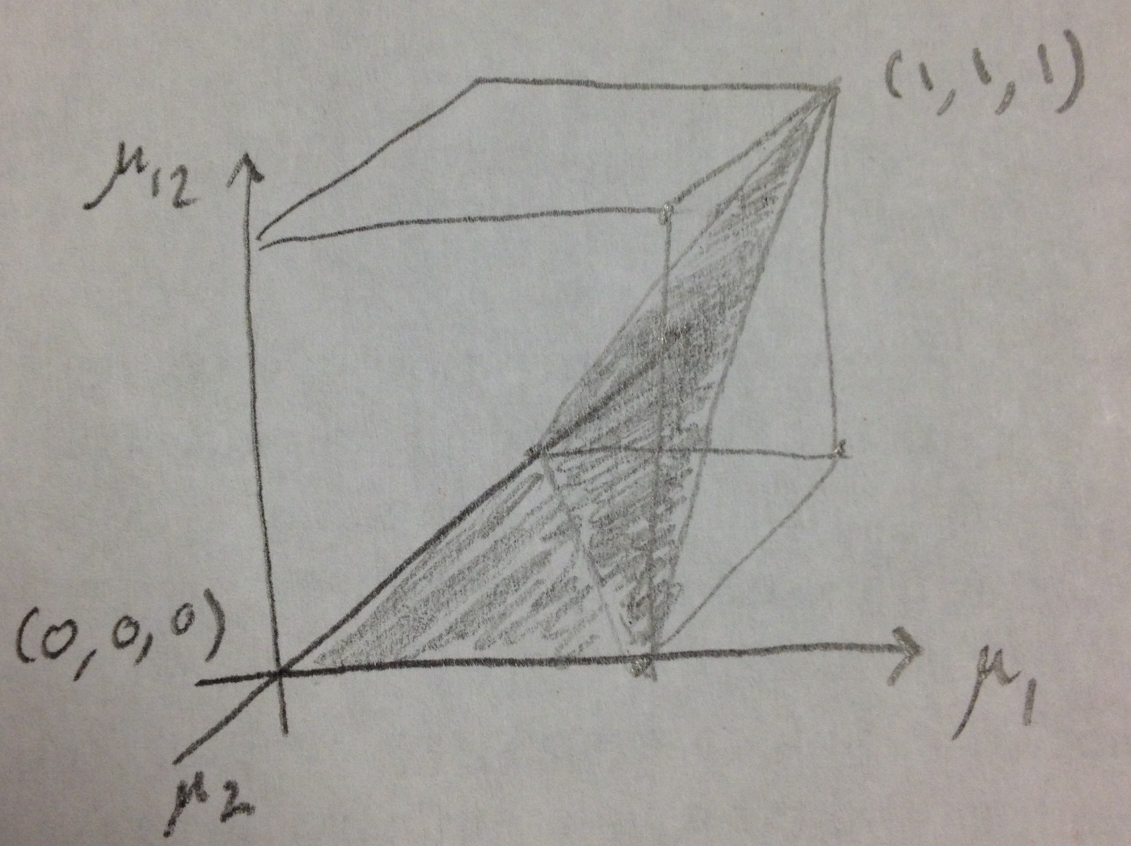
\includegraphics[scale=0. 2]{cube. png}}
\caption{Visualizing Constraints on $\mu$}
\label{mu}
\end{center}
\end{figure}


\begin{figure}[h!]
\begin{center}
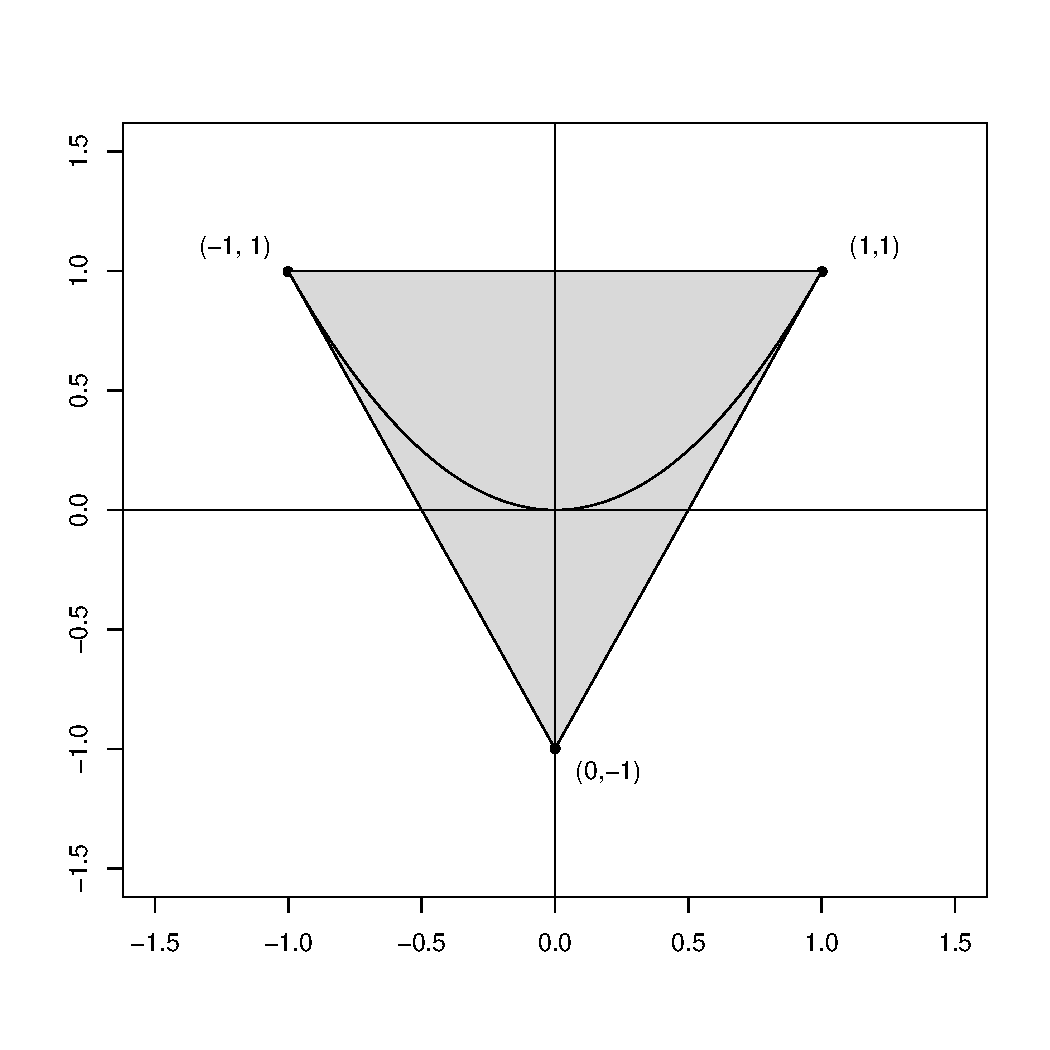
\includegraphics[scale=0. 5]{triangle. pdf}
\caption{Visualizing $\mu_{12}$ when $\mu_1=\mu_2$}
\label{mu2}
\end{center}
\end{figure}

If we take a slice of this convex polytope in Figure \ref{mu} at $\mu_1=\mu_2$,  it is a triangle like the one in Figure \ref{mu2}.  The $x$-axis in the figure is $\mu_1$.  The quadratic curve indicates where $\mu_1^2=\mu_{1, 2}$.  This quadratic function is due to the marginal independence of $\mu_1$ and $\mu_2$.  



\section{Loopy Belief Propogation}



\end{document}

